\section{Mechanical Design}

The basic shape of the HTCC is naturally generated by a combination of 
the dimensions and positions of the surrounding equipment, certain 
required acceptance angles, and the planned focal points of the mirror 
within.  The body will serve primarily as a gas volume container, and 
should have as little material as possible within to obstruct either the 
{\v C}erenkov light, or particles to other detectors.  An overall view of 
the appearance of the HTCC is shown in Fig.~\ref{overall}.
 
%%%%%%%%%%%%%%%%%%%%%%%%%%%%%%%%%%%%%%%%%%%%%%%%%%%%%%%%%%%%%%%%%%%%%%%%%
\begin{figure}[h]
\vspace{0.5cm}
\begin{centering}
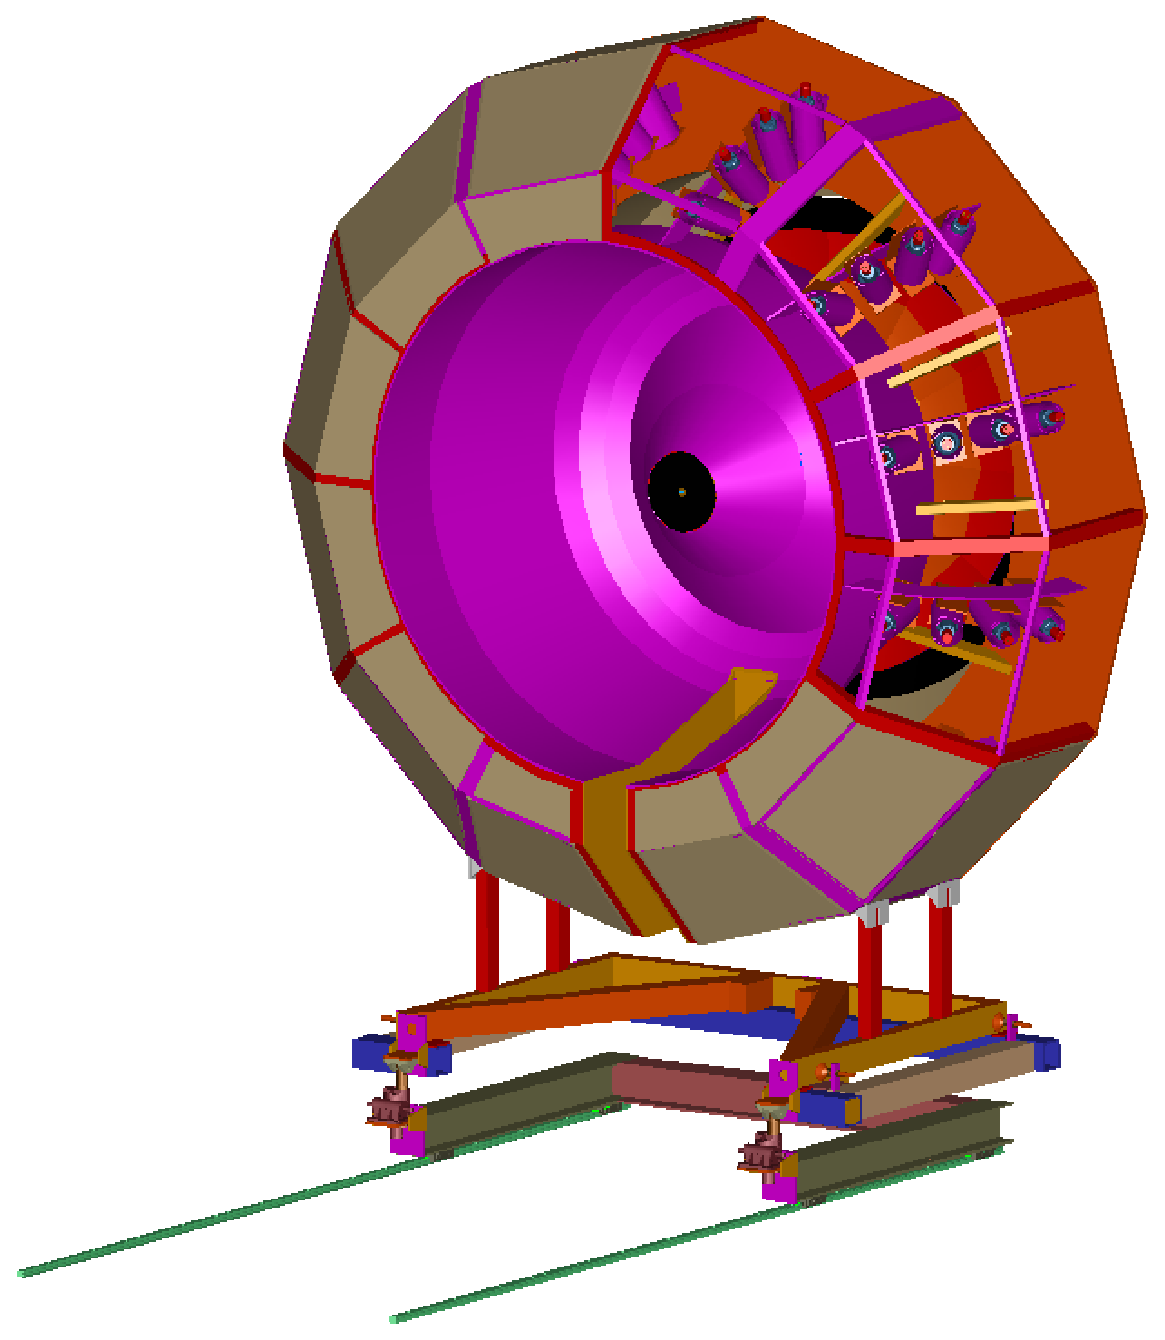
\includegraphics[height=9.0cm,angle=-0]{Mechanical/CD3_Cyril_1.eps}
\hspace{0.1cm}
\caption{\small{Overall appearance of the HTCC viewed from upstream side.}}
\label{overall}
\end{centering}
\end{figure}
%%%%%%%%%%%%%%%%%%%%%%%%%%%%%%%%%%%%%%%%%%%%%%%%%%%%%%%%%%%%%%%%%%%%%%%%%

\subsection{Main Structure}

The geometry of the detector strongly dictates the shape of the HTCC's main 
structure.  The mirror design is a twelve segment combined mirror, and the 
light is focused to twelve banks of 4 photomultiplier tubes per bank.  For 
this mirror, a twelve-sided shell centered around the beamline was designed, 
with space on each segment to mount one row of four PMTs. The shell was 
designed to completely enclose all of the PMTs, mounting hardware, shielding, 
etc..  The strength of the structure comes from the entry cone, the downstream 
mirror housing, and the connecting ribs of rectangular tubing.  The outer 
web of aluminum angles and tees will add to the strength of the unit, but 
is primarily to serve as a frame for panels used to seal the gas volume. The 
structure is still simple, and can be constructed of flat and rolled, 
machined and welded plates, tees, and/or angles of Aluminum (see 
Fig.~\ref{structure}).

%%%%%%%%%%%%%%%%%%%%%%%%%%%%%%%%%%%%%%%%%%%%%%%%%%%%%%%%%%%%%%%%%%%%%%%%%
\begin{figure}[h]
\vspace{0.5cm}
\begin{centering}
\includegraphics[height=9.0cm,angle=-90]{Mechanical/CD3_Cyril_2.eps}
\hspace{0.1cm}
\caption{\small{Mechanical housing of the HTCC.}}
\label{structure}
\end{centering}
\end{figure}
%%%%%%%%%%%%%%%%%%%%%%%%%%%%%%%%%%%%%%%%%%%%%%%%%%%%%%%%%%%%%%%%%%%%%%%%%

\subsection{PMT Mount}

Our original goal was to have the PMTs mounted to the outer surface of 
the HTCC to make maintenance easier, but finding an effective way to seal 
the gas volume, while maintaining some degree of adjustability at each PMT 
within the space available proved to be challenging.  Instead, each PMT, 
Light Concentrator, and any shielding is mounted to one bracket, as shown
in Fig.~\ref{bracket}.  The brackets are mounted to a plate (eight each) as
shown in Fig.~\ref{plate}, and the gas volume of the HTCC is sealed via 
access panels located radially beyond the PMTs as shown in Fig.~\ref{pannels}.
This system is relatively easier and less expensive to manufacture, easy to 
assemble, and each PMT is independently adjustable.

%%%%%%%%%%%%%%%%%%%%%%%%%%%%%%%%%%%%%%%%%%%%%%%%%%%%%%%%%%%%%%%%%%%%%%%%%
\begin{figure}[h]
\vspace{0.5cm}
\begin{centering}
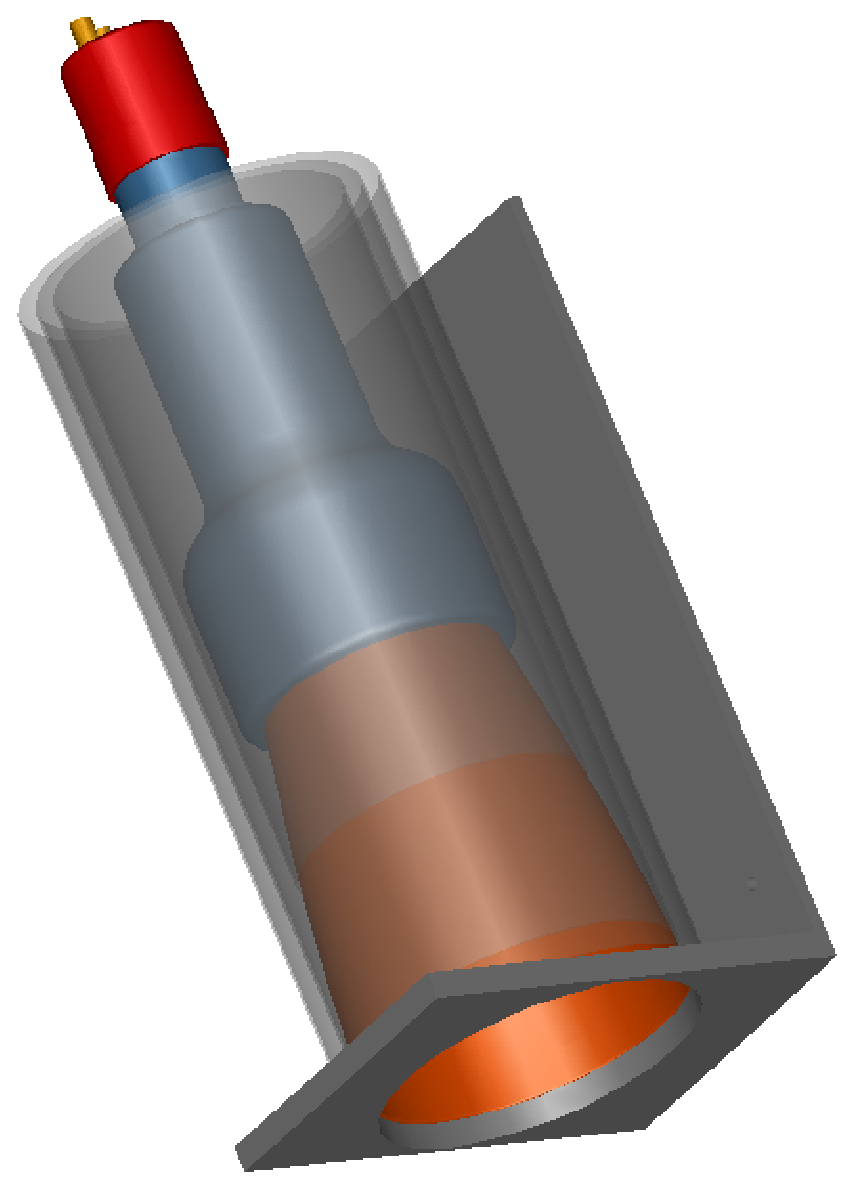
\includegraphics[height=8.0cm,angle=-0]{Mechanical/CD3_Cyril_3.eps}
\hspace{0.1cm}
\caption{\small{Photomultiplier tube with Winston Light Concentrator, 
magnetic shield layers, and mounting block.}}
\label{bracket}
\end{centering}
\end{figure}
%%%%%%%%%%%%%%%%%%%%%%%%%%%%%%%%%%%%%%%%%%%%%%%%%%%%%%%%%%%%%%%%%%%%%%%%%

%%%%%%%%%%%%%%%%%%%%%%%%%%%%%%%%%%%%%%%%%%%%%%%%%%%%%%%%%%%%%%%%%%%%%%%%%
\begin{figure}[h]
\begin{centering}
\includegraphics[height=11.0cm,angle=-90]{Mechanical/CD3_Cyril_4.eps}
\hspace{0.1cm}
\caption{\small{Four photomultiplier tubes with Winston Light Concentrators 
and magnetic shield layers mounted to a plate.}}
\label{plate}
\end{centering}
\end{figure}
%%%%%%%%%%%%%%%%%%%%%%%%%%%%%%%%%%%%%%%%%%%%%%%%%%%%%%%%%%%%%%%%%%%%%%%%%

%%%%%%%%%%%%%%%%%%%%%%%%%%%%%%%%%%%%%%%%%%%%%%%%%%%%%%%%%%%%%%%%%%%%%%%%%
\begin{figure}[h]
\vspace{0.5cm}
\begin{centering}
\includegraphics[height=14cm,angle=-90]{Mechanical/CD3_Cyril_5.eps}
\hspace{0.1cm}
\caption{\small{Access panels covering identical banks of 4 PMTs.}}
\label{pannels}
\end{centering}
\end{figure}
%%%%%%%%%%%%%%%%%%%%%%%%%%%%%%%%%%%%%%%%%%%%%%%%%%%%%%%%%%%%%%%%%%%%%%%%%

\subsection{Mirror Positioning and Alignment}

Using six dual ball-socket adjustment linkages that contact the mirror in 
three places, the mirror can be securely supported and adjusted in all 
directions without inducing any torsional stress upon the mirror.  With 
this system (see Fig.~\ref{linkage}), the mirror would also be protected 
from possible stresses that the main shell may sustain, whether via 
temperature changes, transport, maintenance, or other unforeseen events. 

%%%%%%%%%%%%%%%%%%%%%%%%%%%%%%%%%%%%%%%%%%%%%%%%%%%%%%%%%%%%%%%%%%%%%%%%%
\begin{figure}[h]
\begin{centering}
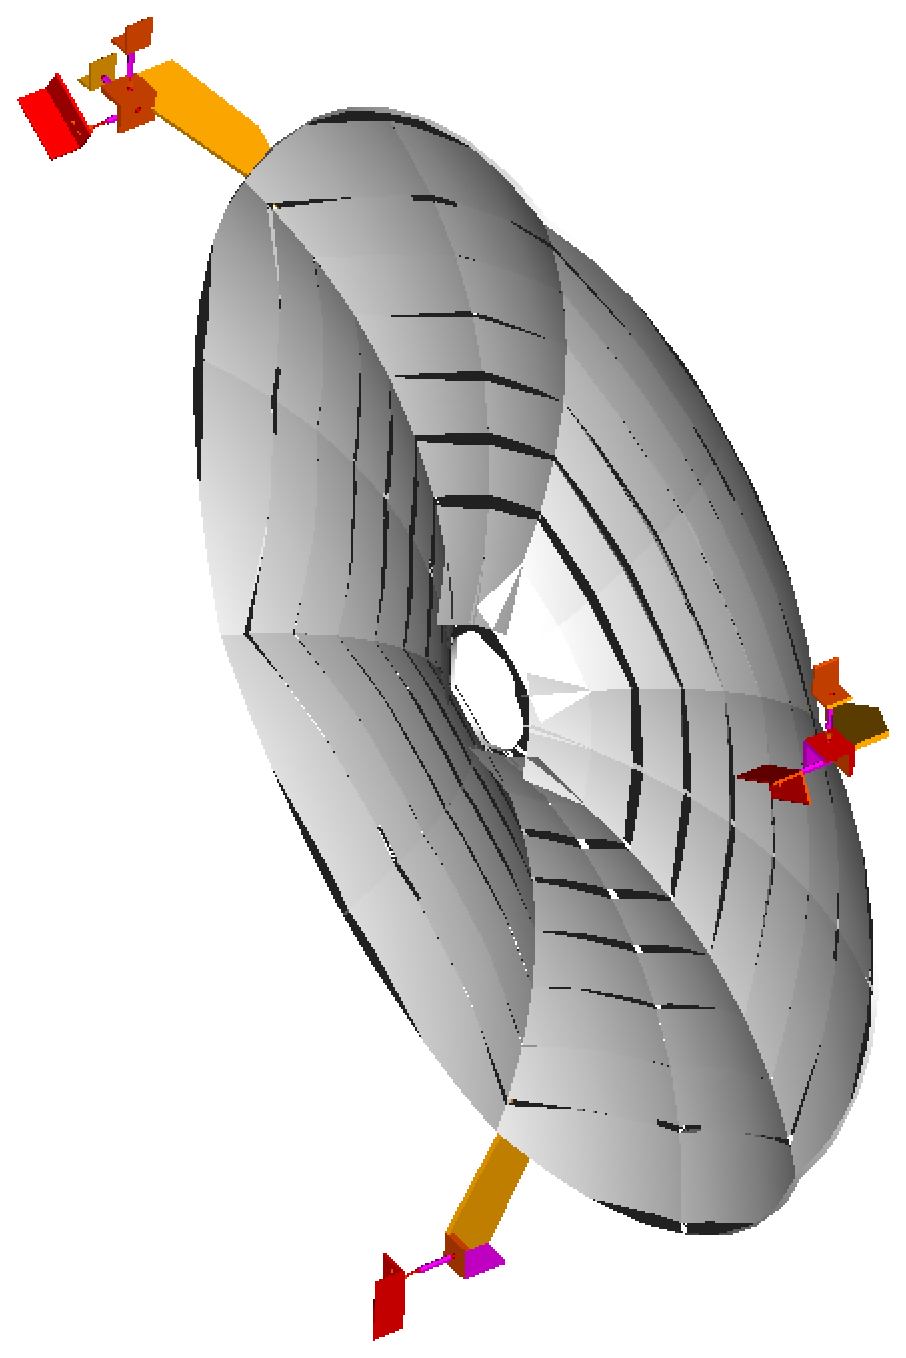
\includegraphics[height=7.0cm,angle=-0]{Mechanical/CD_2_Cyril_6.eps}
\hspace{0.1cm}
\caption{\small{HTCC mirror supported in three places using adjustment 
linkages.}}
\label{linkage}
\end{centering}
\end{figure}
%%%%%%%%%%%%%%%%%%%%%%%%%%%%%%%%%%%%%%%%%%%%%%%%%%%%%%%%%%%%%%%%%%%%%%%%%

\subsection{Upstream and Entry}

The upstream end of the HTCC must wrap closely around the CTOF and 
solenoid magnet, to both avoid interfering with the light paths, and to 
allow for the greatest possible acceptance angle from the target. This 
results in a cup shape that reaches from the outside of the solenoid magnet, 
around the downstream CTOF light guides, with a cone in the center that 
follows the light guides back in toward the center of the solenoid, stopping 
just before the SVT.  This entry cone must be as thin as possible to retain 
every available degree of entry angle.  Currently, the optimized entry 
acceptance angle of 36$^\circ$ is limited by the solenoid shape and the 
position of the CTOF light guides.  This angle is only achievable using 
equipment clearances as low as 0.20~in, and an entry cone thickness of 
0.040~in.  At this thickness, the cone could be made of aluminum or a 
carbon composite; it is not a structural member, and only needs to be 
strong enough to support itself and the entry window.  A view of the entry 
structure is shown in Fig.~\ref{entry}.

%%%%%%%%%%%%%%%%%%%%%%%%%%%%%%%%%%%%%%%%%%%%%%%%%%%%%%%%%%%%%%%%%%%%%%%%%
\begin{figure}[h]
\begin{centering}
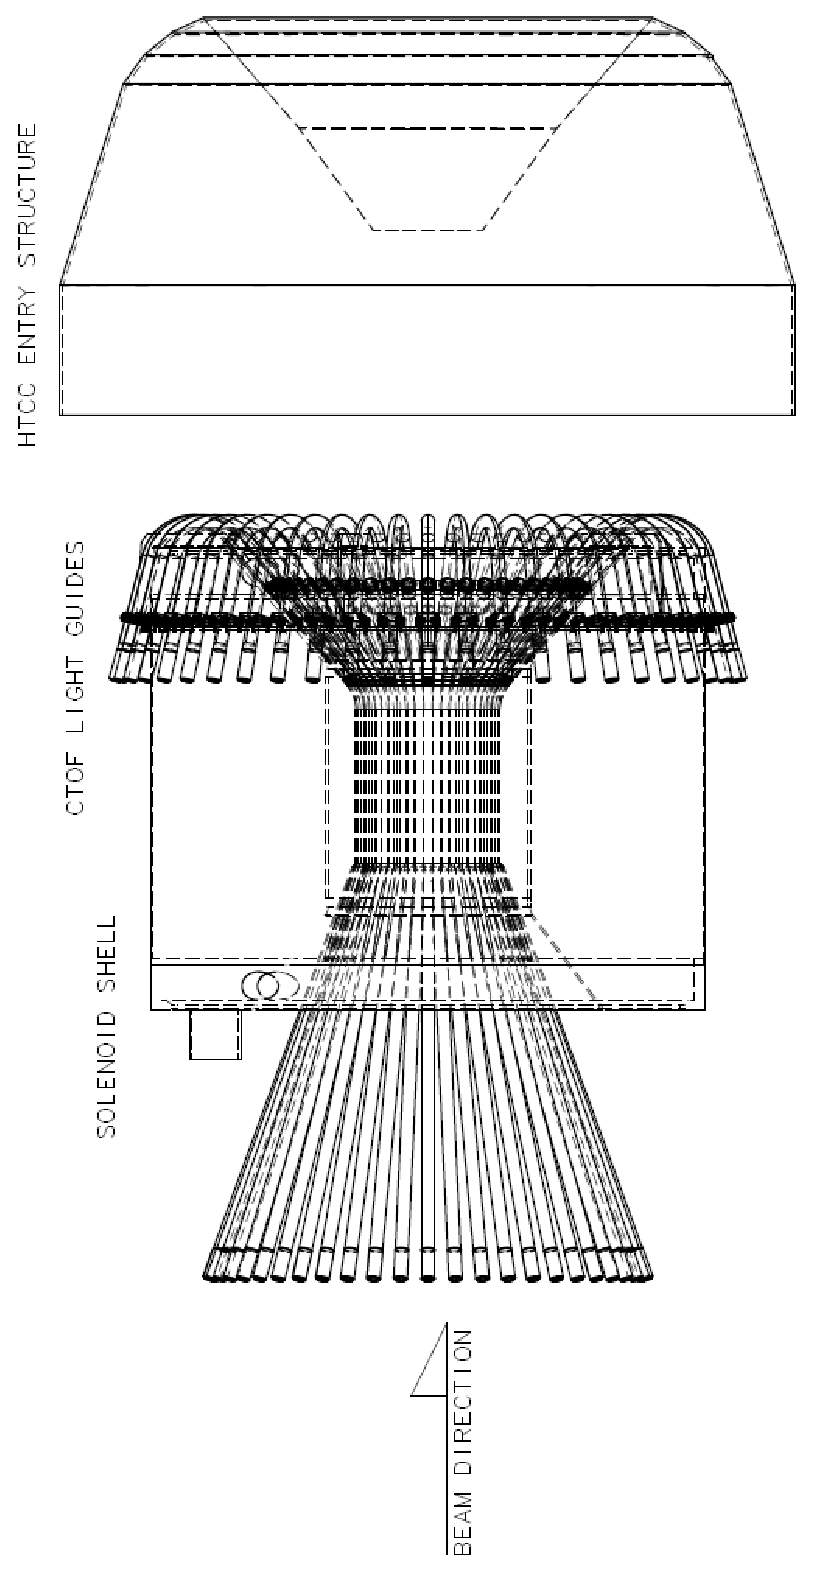
\includegraphics[height=16.0cm,angle=270]{Mechanical/CD3_Cyril_7.eps}
\hspace{0.1cm}
\caption{\small{HTCC mechanical entry structure.}}
\label{entry}
\end{centering}
\end{figure}
%%%%%%%%%%%%%%%%%%%%%%%%%%%%%%%%%%%%%%%%%%%%%%%%%%%%%%%%%%%%%%%%%%%%%%%%%

\subsection{Exit Scheme}

From the portion of the shell where the photomultiplier tubes are mounted, 
a cylindrical tube reaches downstream to house and support the mirror and 
adjustment fixtures, and finally interfaces with the exit window.  The 
exit window of the HTCC is located approximately 0.5~in past the mirror of 
the HTCC. It must allow up to 41$^\circ$ particles to pass through the gas 
volume unobstructed.  Because of the shape of the next detector in the 
beamline (Region~1 drift chamber), the outer edge of the HTCC exit window 
must be beveled to avoid interference with Region~1, see Fig.~\ref{exit}.

%%%%%%%%%%%%%%%%%%%%%%%%%%%%%%%%%%%%%%%%%%%%%%%%%%%%%%%%%%%%%%%%%%%%%%%%%
\begin{figure}[h]
\vspace{1cm}
\begin{centering}
\includegraphics[height=15.0cm,angle=-90]{Mechanical/CD3_Cyril_8.eps}
\hspace{0.1cm}
\vspace{1cm}
\caption{\small{View of the mechanical components of the outer shell.}} 
\label{exit}
\end{centering}
\end{figure}
%%%%%%%%%%%%%%%%%%%%%%%%%%%%%%%%%%%%%%%%%%%%%%%%%%%%%%%%%%%%%%%%%%%%%%%%%
